\section{Analysing output}
\begin{frame}[fragile]{\Queso\ output}
  \begin{itemize}
    \item At this point, you should be able to see your samples.
    \item Are they correct?
    \item Should look like white noise
    \item Steps or large meanderings is considered transient behaviour
    \item An initial transient period is ok (see later) but it should settle
      down
    \item If there is an initial transient period, do not include this period
      when calculating mean, variance, other moments
    \item There are more quantitative convergence metrics: autocorrelation,
      Geweke, effective sample size, Raftery and Lewis, Heidelberger and Welch,
      Gelman and Rubin.
    \item See here for details: \url{https://support.sas.com/documentation/cdl/en/statug/63033/HTML/default/viewer.htm#statug_introbayes_sect008.htm}
  \end{itemize}
\end{frame}

\begin{frame}[fragile]{\Queso\ output: Autocorrelation}
  Autocorrelation of chain:
  \begin{figure}
    \begin{center}
      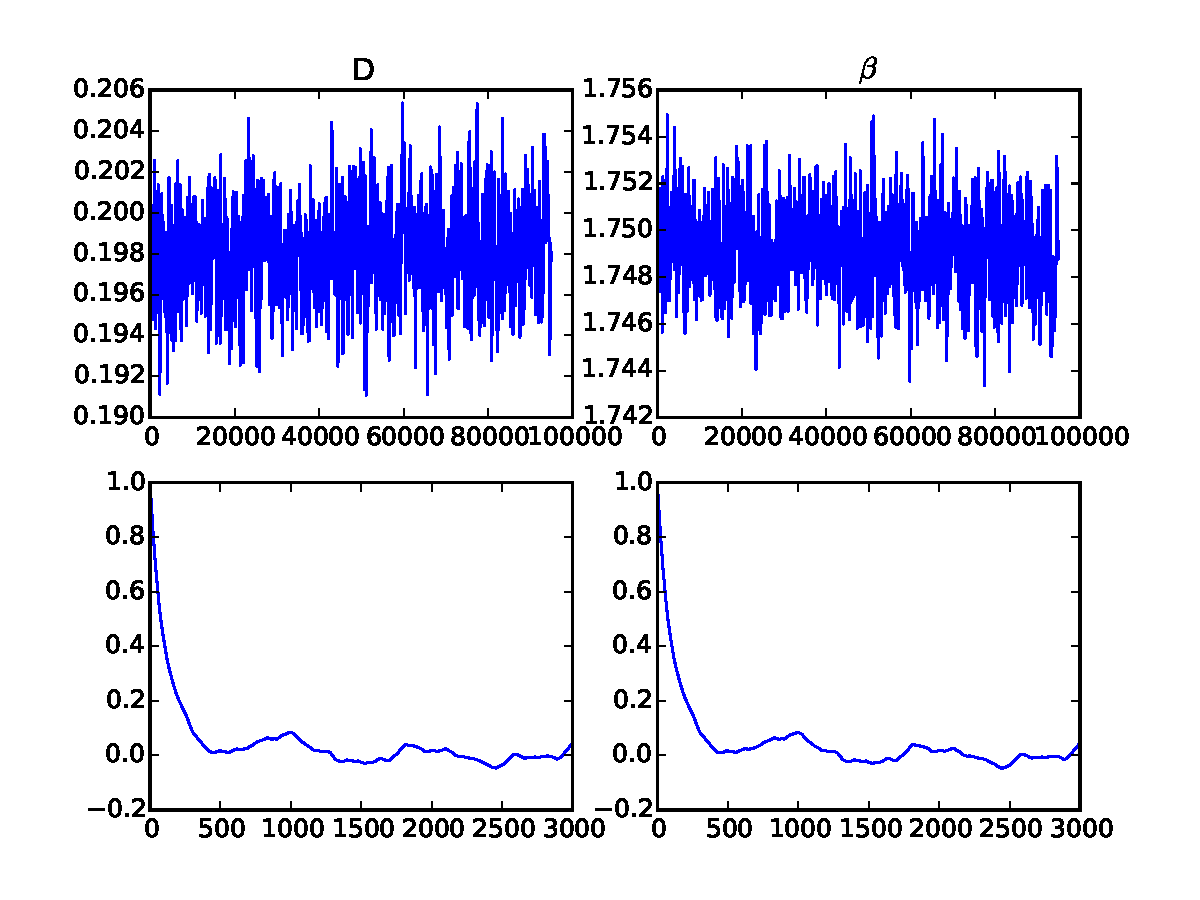
\includegraphics[width=0.85\textwidth]{autocorrs.pdf}
    \end{center}
  \end{figure}
\end{frame}

\begin{frame}[fragile]{\Queso\ output: Autocorrelation}
  Autocorrelation of white noise:
  \begin{figure}
    \begin{center}
      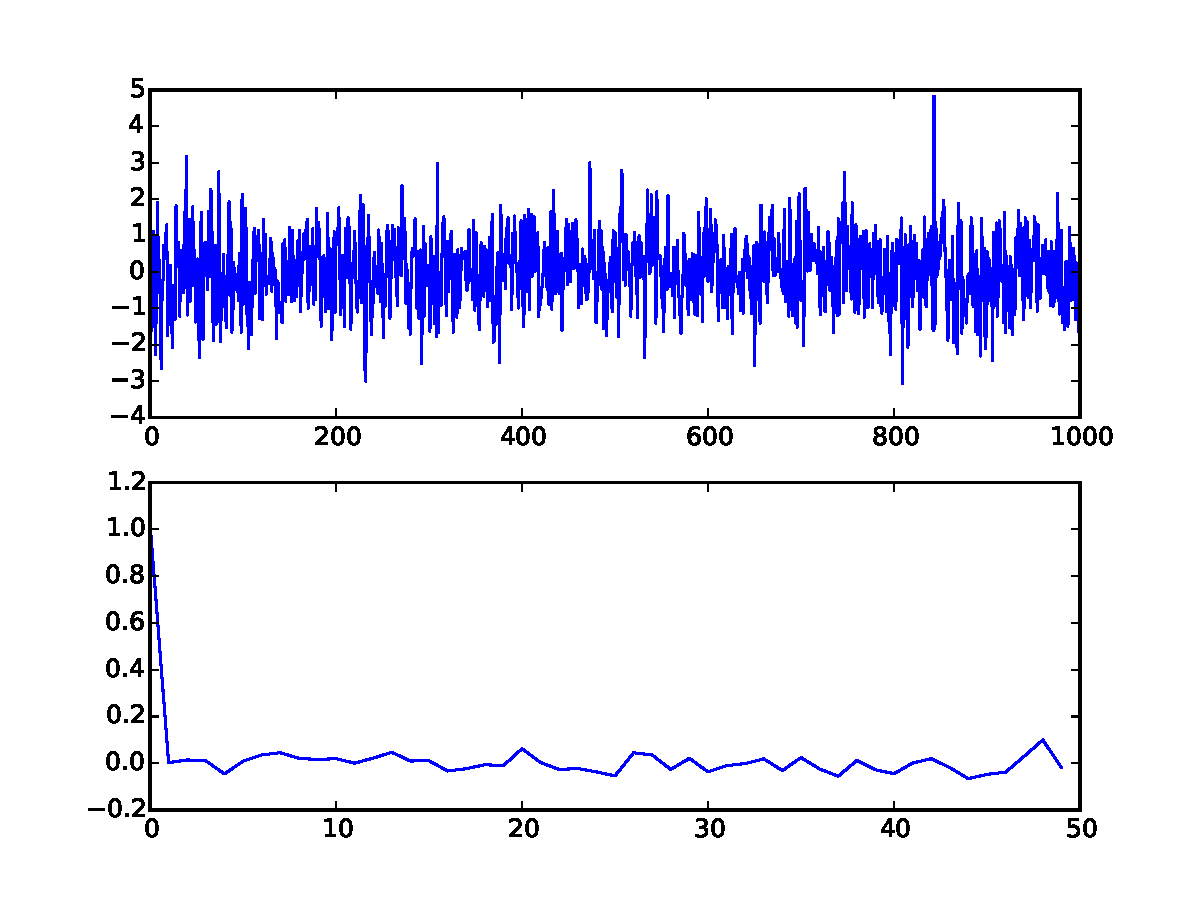
\includegraphics[width=0.85\textwidth]{autocorrs_white_noise.pdf}
    \end{center}
  \end{figure}
  Time taken for autocorrelation to decay is a measure of Markov chain mixing
  efficiency.  `Mixing' is how well the Markov chain explores the state space.
\end{frame}

\begin{frame}[fragile]{\Queso\ output: Geweke diagnostic}
  Take averages of chunk of samples from beginning and end separately:
  \begin{align*}
    \bar{D}_1 &= \frac{1}{n_1} \sum_{i=1}^{n_1} D_i \\
    \bar{D}_2 &= \frac{1}{n_2} \sum_{i=n - n_2 + 1}^{n} D_i
  \end{align*}
  The distribution of the random variable $\bar{D}_1 - \bar{D}_2$ converges to
  a normal distribution with mean zero.
\end{frame}

\begin{frame}[fragile]{\Queso\ output: Geweke diagnostic}
  \begin{figure}
    \begin{center}
      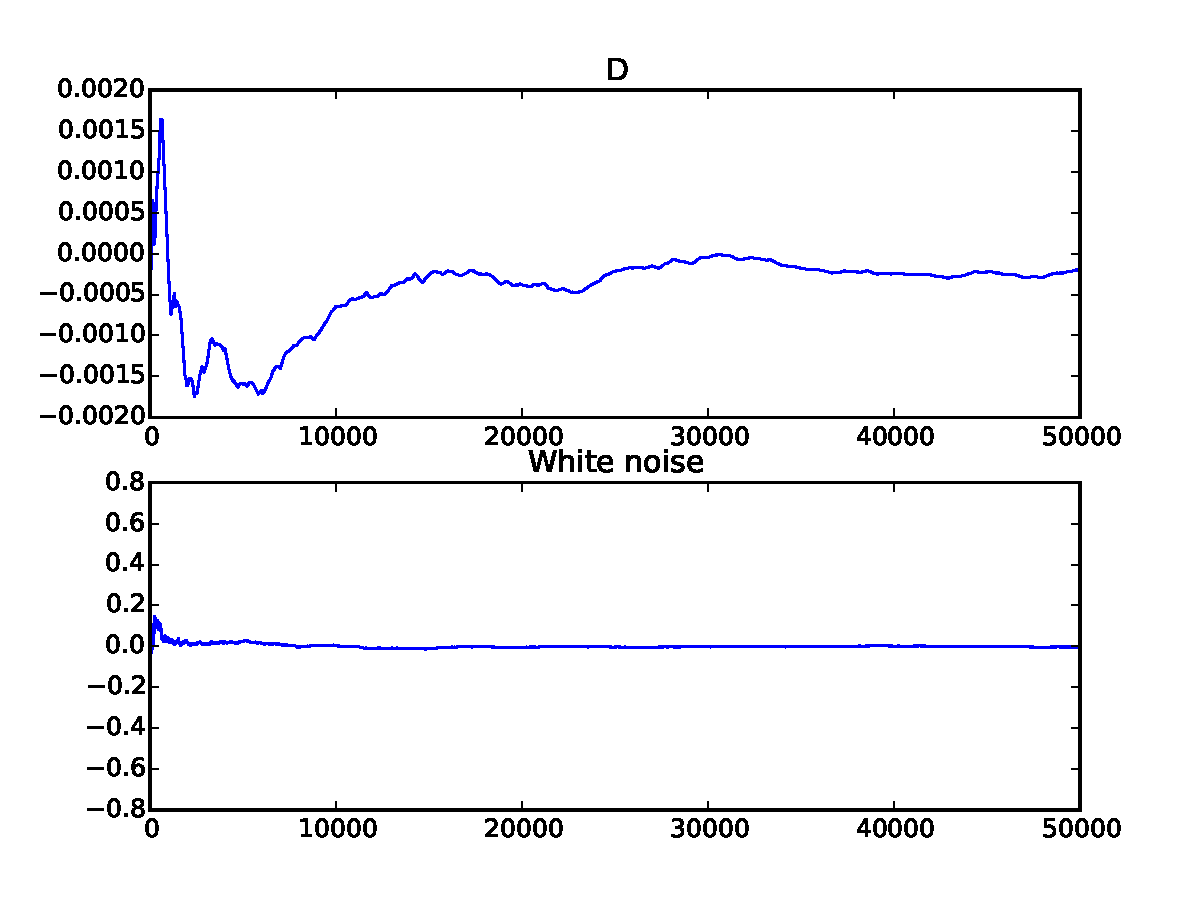
\includegraphics[width=0.85\textwidth]{geweke.pdf}
    \end{center}
  \end{figure}
\end{frame}

\begin{frame}[fragile]{Other \Queso\ output}
  \begin{itemize}
    \item Other useful output is produced by \Queso.
    \item Should be reasonably obviously named, but:
      \begin{itemize}
        \item log-likelihood values at each sample in the chain:
          \texttt{ip\_raw\_chain\_loglikelihood.m}
        \item log-target values at each sample in the chain:
          \texttt{ip\_raw\_chain\_logtarget.m}
        \item General diagnostic information and logging information that
          \Queso\ encounters:
          \texttt{display\_sub0.txt}
        \item Algorthmic information about the inverse problem:
          \texttt{sipOutput.m}
          \begin{itemize}
            \item Proportion of rejected samples is written here
          \end{itemize}
      \end{itemize}
  \end{itemize}
\end{frame}
